\chapter{Esperimento pilota}

%immagine Immagini/pilota/cardinalita_problema.png -> immagine con l'algorimo di forza bruta che funziona male a causa del tipo di variabile
%Immagini/pilota/sol.png -> immagine con la soluzione ottima del problema (di tutti gli algoritmi) 
%Immagini/pilota/tempo_sparso.png -> immagine con il tempo di esecuzione dei cinque algoritmi per i grafi sparsi
%Immagini/pilota/tempo_denso.png -> immagine con il tempo di esecuzione dei cinque algoritmi per i grafi densi

Prima di procedere con la campagna sperimentale vera e propria, è stato condotto un esperimento pilota: una sperimentazione volutamente piccola e veloce, con l'obiettivo non di rispondere alle domande di ricerca del Capitolo~3, ma di verificare che l'infrastruttura sperimentale (generazione dei grafi, esecuzione dei cinque algoritmi, raccolta dei risultati) funzioni correttamente prima di investirci sopra ore di calcolo. Come si vedrà, questo obiettivo si è rivelato tutt'altro che superfluo.

\section{Configurazione}

Sono stati generati dieci grafi con il generatore Erdos-Renyi di cinque dimensioni ($n = 10, 15, 20, 25, 30$), ciascuna nei due livelli sparso e denso. 
Su ciascuno dei dieci grafi sono stati eseguiti tutti e cinque gli algoritmi: forza bruta, branch-and-bound, ILP (Gurobi), 2-approssimato e greedy.

\section{Primo tentativo: un bug nella forza bruta}

Il primo tentativo di esecuzione del pilot ha subito mostrato perché la fase pilota non è un passaggio superfluo. 
L'implementazione della forza bruta smetteva di funzionare correttamente in corrispondenza di $n=30$, come si evince dalla figura~\ref{fig:problema}. 
La causa era un errore di tipizzazione nella variabile usata per enumerare i sottoinsiemi di vertici. 
Infatti, la maschera di bit era rappresentata con un intero a 32 bit con segno, insufficiente a contare fino a $2^{30}$ sottoinsiemi senza andare in overflow.
\begin{figure}[htbp]
    \centering
    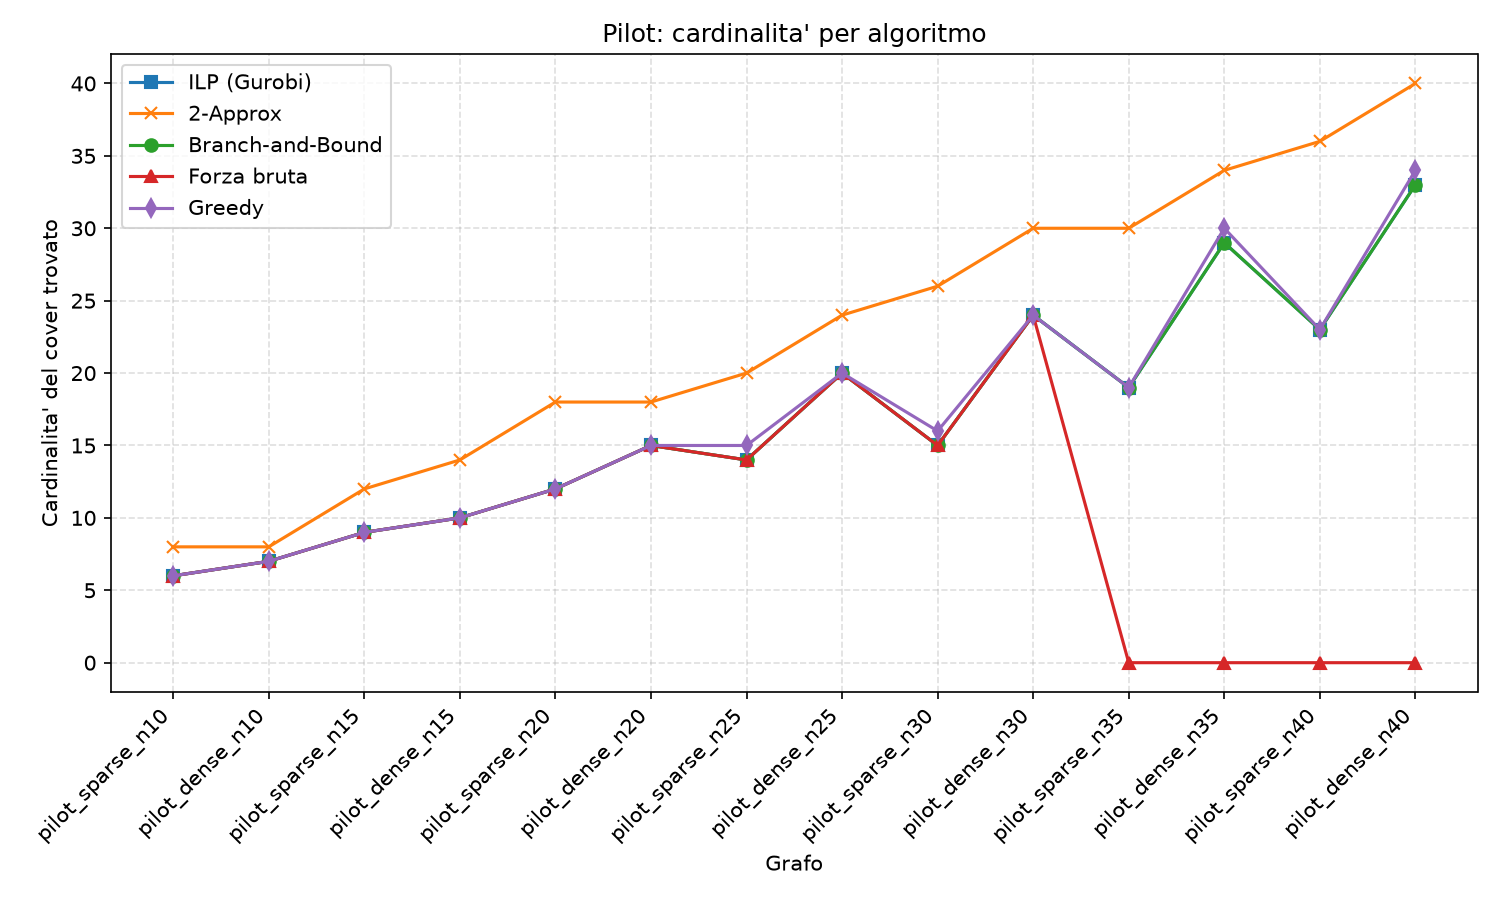
\includegraphics[width=0.9\linewidth]{Immagini/pilota/cardinalita_problema.png }
    \caption{Cardinalità del cover trovato da ciascun algoritmo, sui dieci grafi del pilot.}
    \label{fig:problema}
\end{figure}

\begin{lstlisting}[language=C++, caption={Versione difettosa: maschera a 32 bit con segno}]
for (int mask = 0; mask < (1 << n); mask++) {
    // ...
}
\end{lstlisting}

La correzione è consistita nel passare a un tipo a 64 bit senza segno, sufficiente a rappresentare correttamente $2^n$ anche per valori di $n$ ben oltre quelli usati in questo pilot.

\begin{lstlisting}[language=C++, caption={Versione corretta: maschera a 64 bit senza segno}]
for (unsigned long long mask = 0; mask < (1ULL << n); mask++) {
    // ...
}
\end{lstlisting}

Questo bug è precisamente il tipo di problema che un esperimento pilota è pensato per intercettare. Un errore che sarebbe potuto passare inosservato se il primo test fosse stato direttamente la campagna sperimentale su larga scala, con il rischio di scoprire i dati compromessi solo a posteriori, a ore di calcolo già spese.

\section{Secondo tentativo: risultati}

Con la correzione applicata, il pilot è stato rieseguito. La Figura~\ref{fig:pilot-cardinalita} riporta la cardinalità del cover trovato da ciascun algoritmo su ciascuno dei dieci grafi.

\begin{figure}[htbp]
    \centering
    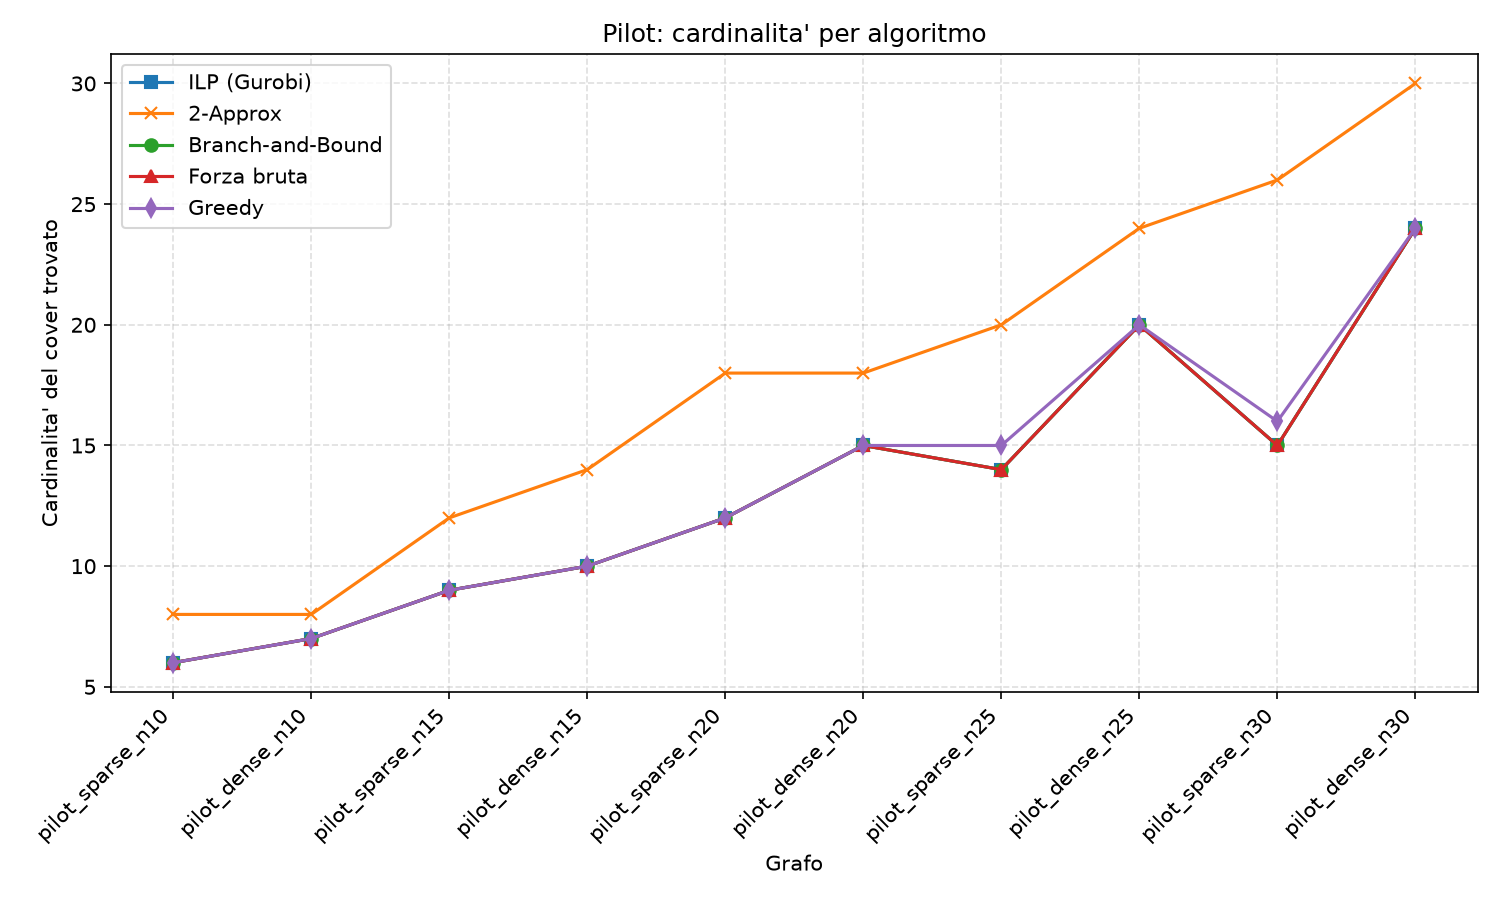
\includegraphics[width=0.9\linewidth]{Immagini/pilota/sol.png }
    \caption{Cardinalità del cover trovato da ciascun algoritmo, sui dieci grafi del pilot.}
    \label{fig:pilot-cardinalita}
\end{figure}

Il risultato atteso si conferma. 
I tre algoritmi esatti (forza bruta, branch-and-bound, ILP) restituiscono sempre la stessa cardinalità, su tutti e dieci i grafici. 
Gli algoritmi greedy e 2-approssimato trovano invece una soluzione valida ma non sempre ottima. 
Il greedy resta quasi sempre molto vicino al valore ottimo o lo raggiunge, mentre il 2-approssimato se ne allontana in modo più marcato e sistematico, restando comunque sempre entro il fattore 2 dimostrato nel Capitolo~1.

\section{Prestazioni}

Le Figure~\ref{fig:pilot-tempo-sparso} e~\ref{fig:pilot-tempo-denso} riportano il tempo di esecuzione dei cinque algoritmi, rispettivamente sui grafi sparsi e su quelli densi, in scala logaritmica.

\begin{figure}[htbp]
    \centering
    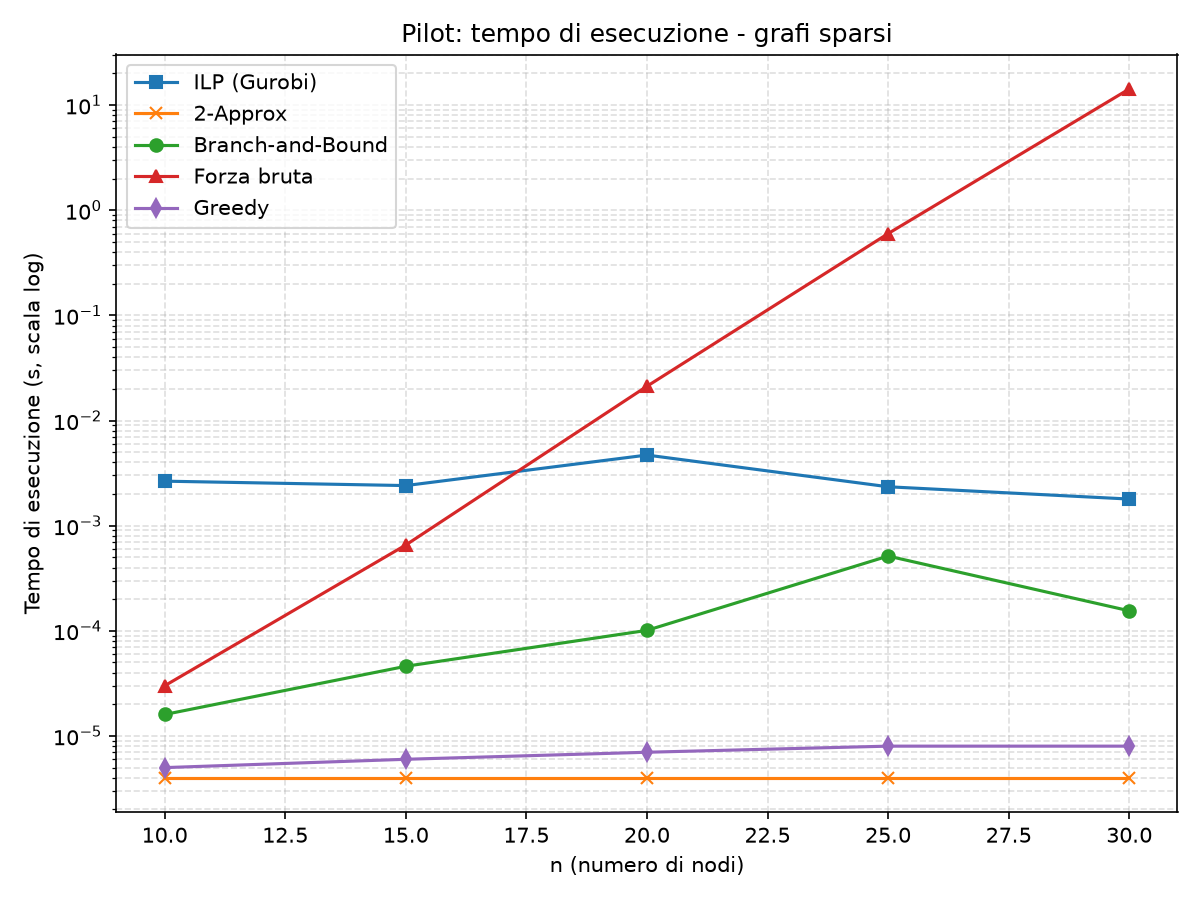
\includegraphics[width=0.9\linewidth]{Immagini/pilota/tempo_sparso.png}
    \caption{Tempo di esecuzione dei cinque algoritmi sui grafi sparsi.}
    \label{fig:pilot-tempo-sparso}
\end{figure}

\begin{figure}[htbp]
    \centering
    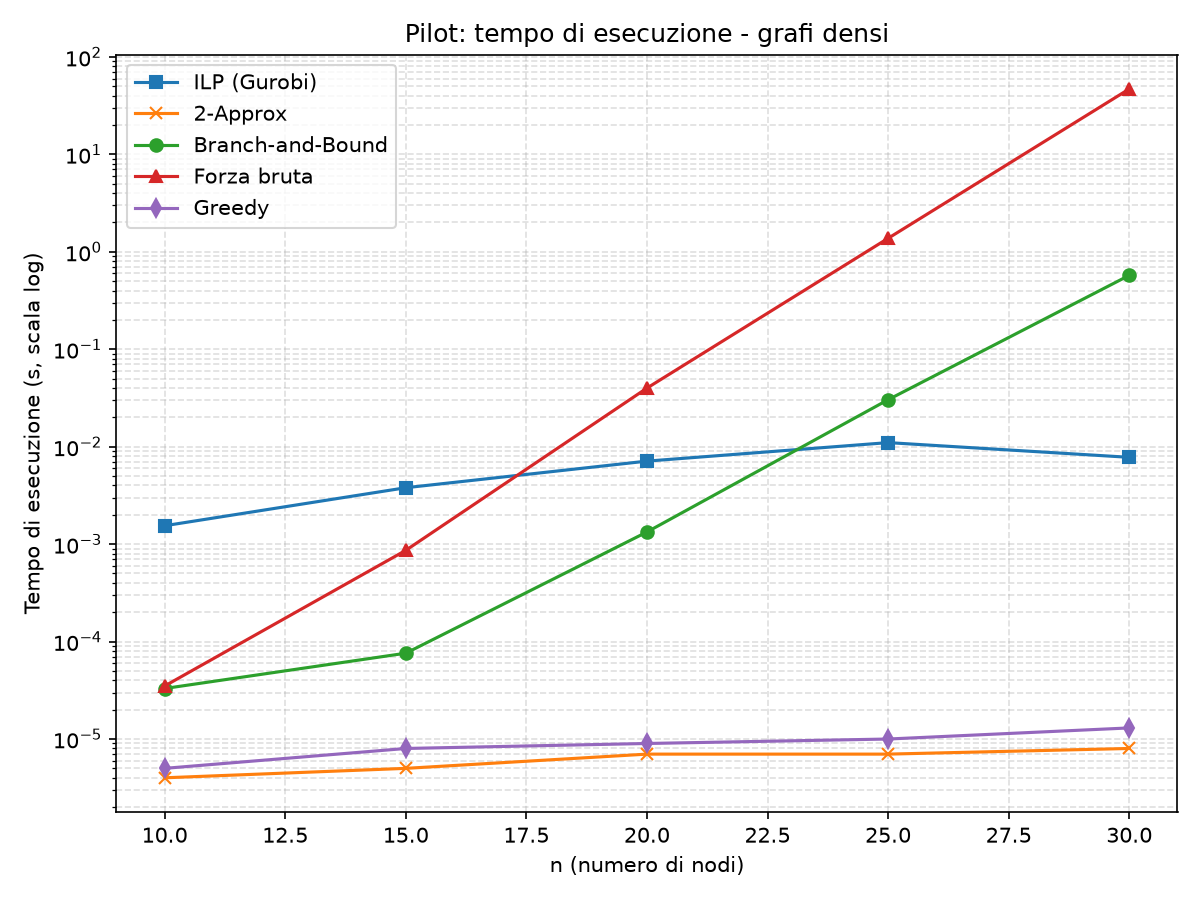
\includegraphics[width=0.9\linewidth]{Immagini/pilota/tempo_denso.png}
    \caption{Tempo di esecuzione dei cinque algoritmi sui grafi densi.}
    \label{fig:pilot-tempo-denso}
\end{figure}

Una prima osservazione, valida per tutti e cinque gli algoritmi, è che i tempi sui grafi sparsi sono sistematicamente inferiori a quelli sui grafi densi a parità di $n$. 
È il comportamento atteso. Infatti, a parità di numero di vertici, un grafo più denso ha più vincoli da soddisfare e uno spazio di ricerca meno facilmente potabile.

Guardando l'andamento di ciascun algoritmo al crescere di $n$:

\begin{itemize}
    \item \textbf{Forza bruta}: crescita nettamente esponenziale in entrambi i grafici, coerente con la complessità $O(2^n \cdot (|V|+|E|))$ discussa nel Capitolo~1.    
    \item \textbf{Branch-and-bound}: anch'esso di andamento esponenziale nel caso peggiore, ma con una base molto più favorevole grazie alla potatura. 
    \item \textbf{ILP (Gurobi)}: Il grafico mostra un andamento quasi piatto, che potrebbe suggerire un comportamento polinomiale, ma l'ILP resta un metodo esatto per un problema NP-hard, e nel caso peggiore la sua complessità è comunque esponenziale quanto quella del branch-and-bound, non polinomiale. Quello che i dati mostrano è che, nel range di $n$ testato, non si è ancora raggiunto il punto in cui il motore inizia a degradare. È un'osservazione che verrà approfondita nella campagna sperimentale vera.
    \item \textbf{Greedy e 2-approssimato}: questi sono polinomiali, non solo empiricamente ma per costruzione ($O(|V|+|E|)$, Capitolo~1), ed è esattamente ciò che si osserva. I tempi sono dell'ordine dei microsecondi, praticamente costanti su tutto il range testato, ordini di grandezza sotto tutti e tre i metodi esatti.
\end{itemize}
